\graphicspath{{images/}}

\section{\thesection~Methods}
\label{sec:methods}

To analyse QFA data I created a Python package (``CANS'') for model
composition, model simulation, parameter inference, and visualisation
of results. It accepts timecourse data from QFA using any size
rectangular array. CANS can produce SBML models to document fitting
results which can be validated independently using a variety of
tools. It is relatively simple to create new models, similar in form
to the competition model, containing reactions between species within
cultures or between neighbouring cultures. These can also be simulated
and fit. (Methods for making initial guesses are model specific.) The
CANS package is available for download at (github).

\subsection{\thesubsection~Tools, solving, and fitting}

To analyse QFA data I created a Python package (``CANS'') for model
composition, model simulation, parameter inference, and visualisation
of results. It accepts timecourse data of culture density for any size
rectangular array. I use QFA data after processing with Colonyzer
\citep{Lawless2010}. Colonyzer processes series of time-stamped
whole-plate images and uses integrated optical density measurements as
a proxy for cell density to produce timecourses for all cultures on a
plate. I use these cell density estimates, with arbitrary units,
throughout my analysis.

% read in data using pandas probably don't need to know how I read in
% csv files

I solved models by one of two methods. The first was slower and used
SciPy's integrate.odeint. I optimised solving of the competition model
with this method by vectorising (\ref{eq:competition_model} using
NumPy. For solving a plate of 384 cultures with 10 unevenly spaced
time points I found a \(\sim\)10x further increases in speed by using
Python bindings for the package libRoadRunner. libRoadRoadrunner
requires models to be written in SBML so I wrote code using the
libSBML Python API to automatically generate SBML versions of the
compettion model for any size plate.
% //I could go into more detail about how models are defined// but
% maybe this is not needed.
I solved SBML models using libroadrunner's RoadRunner.simulate. Unlike
SciPy's odeint, RoadRunner can only simulate at even time intervals.
To fit QFA cell observations, which are not taken at even intervals,
requires simulated cell amounts at the observed timepoints. For the
analysis in (P15 section), where each timecourse has only 10
timepoints, I simulated repeatedly between timepoints. For the
analysis in (Stripes section), each timecourse had \(sim\)30
timepoints and this made solving between timepoints slow.

To increase speed I splined data using SciPy's interpolate simulated
using 15 evenly spaced timepoints over the course of observations and
used these to simulate with one call to RoadRunner's
RoadRunner.simulate.

I used SciPy's interpolate.splrep to make a 5th order B-spline of cell
density timecourses with smoothing condition \(s=1.0\). I evaluted the
spline for cell density using SciPy's interpolate.splev at 15 evenly
spaced intervals from time zero to the time of the last QFA
observation. I the solved these timecourses using libRoadRunner
without having to simulate between timepoints.



% tolerances - These tolerances returned estimated parameters with a
% high precision when using simulated data sets.

%initial amounts
%time points and splining

% Displayed output using matplotlib

% Automatic SBML model composition
% Should I include a code example of defining a model?

% SolvingThis uses libRoadRunners

\subsection{\thesubsection~Parameter conversion}

(Could move to discussion: The identity of the
nutrient molecule is unknown and it is not clear whether metabolism of
the nutrient molecule will have a significant effect. If necessary a
metabolism reaction could also be modelled.)\\

When \(k_{n}\) is set to zero, the competition model
(\ref{eq:competition_model}) reduces to the mass action logistic model
which and has the same sigmoidal solution as the standard logistic
model. In this limit, it is possible to equate cells of both models
and convert parameters using (\ref{eq:conversion}) (see Conor's blog
for a derivation).
% Derivation or link to blog.
\begin{subequations}
  \label{eq:conversion}
  \begin{align}
    &r_{i} = b_{i}(C_{t_{0}} + N_{t_{0}})\\
    &K = (C_{t_{0}} + N_{t_{0}})
    % &r = b(C_{t_{0}} + N_{t_{0}})\\
    % &K = (C_{t_{0}} + N_{t_{0}})
  \end{align}
\end{subequations}
%
The reaction equation of the competition model (\ref{eq:reaction})
assumes that all nutrients are converted to cells. This implies that
cultures starting with the same amount of nutrients reach the same
final amount of cells. To fit the mass action logistic model, it is
necessary to allow \(N_{t_{0}}\) to vary for each culture which is not
physical. In this case, the mass action logistic model has the same
number of parameters (769) as the standard logistic model. (Probably
repetition: When I fit the competition model I collectively fit the
timecourses of all cultures on a plate using a plate level
\(N_{t_{0}}\) and 387 parameters.)
%
Figure~\ref{fig:correction} shows fits of a single culture on a larger
16x24 format plate using both models. This culture grew faster than
its neighbours (not shown) and, according to the competition model,
competed for more nutrients.
%
Figure~\ref{fig:correction}a shows the mass-action logistic model fit
where \(N_{t_{0},i}\) is estimated as being approximately equal to the
final cell amount, or carrying capacity \(K_{i}\).
%
Figure~\ref{fig:correction}b shows the competition model fit with a
plate level \(N_{t_{0}}\) and \(kn > 0\). Re-simulating with \(k_{n}\)
set to zero to gives the dashed curves that are equivalent to the
logistic model and which we would be observe if there were no
competition. Competition can therefore be corrected for by converting
competition model estimates of \(b_{i}\), \(C_{t_{0}}\), and
\(N_{t_{0}}\) to independent model \(r_{i}\) and \(K_{i}\) by
(\ref{eq:conversion}).
% This produces the correction in \(r\) and \(K\) between the two fits
% (see Figures~\ref{fig:correction}) and allows direct comparison
% between competition and logistic model estimates.
%

In the competition model, \(C_{t_{0}}\) and \(N_{t_{0}}\) are the same
for all cultures on a plate. Therefore, by the conversion equations
(\ref{eq:conversion}), all cultures have the same carrying capacity
\(K\) and all \(b_{i} \propto r_{i}\) by the same factor. Similarly
all \(b_{i} \propto MDR_{i}\) by the same factor and \(MDP\) is the
same for all cultures (see equation~\ref{eq:MDR_MDP}). \(b_{i}\) is
therefore equivalent to the QFA fitness estimates currently in use
(see e.g. \citet{Addinall2011} and \citet{qfa2016}). This makes
\(b_{i}\) an ideal fitness estimate for the competition model; we need
not convert to logistic model parameters to compare the fitness
rankings of cultures on the same plate. To compare competition model
fitness rankings between different plates we can of course use
\(b_{i}\). However, this is not equivalent to comparing \(r_{i}\) or
\(MDR_{i}\) as different plates may have different \(C_{t_{0}}\) and
\(N_{t_{0}}\).

\begin{Figure}
  \centering
  \graphicspath{{images/correction/}}
  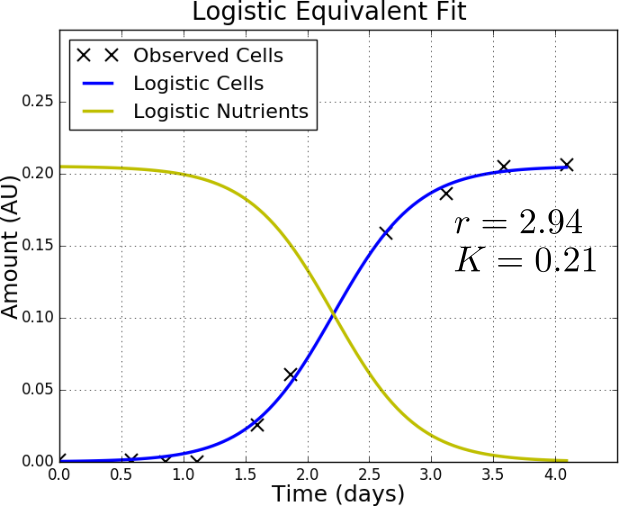
\includegraphics[width=\linewidth]{final/logistic}
  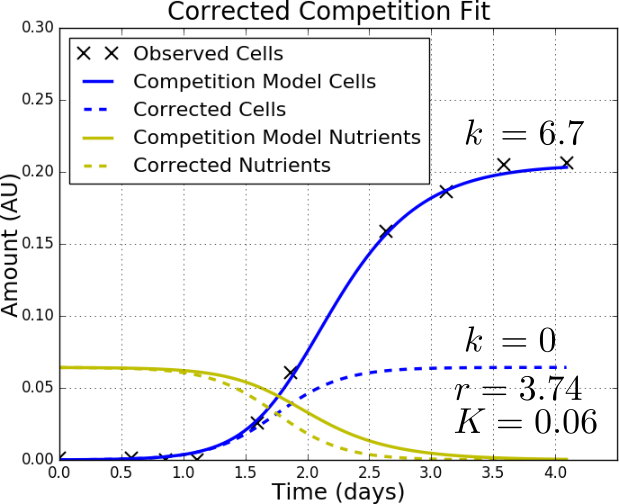
\includegraphics[width=\linewidth]{final/competition}
  \captionof{figure}{\textbf{Using the competition model to correct
      for competition.} Fits are to culture (R10, C3) of P15 which
    grew faster and reached a higher final cell density than its
    neighbours (not shown). According to the competition model, this
    is because this culture competed for more nutrients. To reach the
    same final cell density, the logistic equivalent model requires a
    higher amount of starting nutrients for this culture and a
    different amount for each neighbour. The correction to the
    competition model simulates how growth would have appeared without
    competition and allows us to return parameters \(r\) and \(K\) of
    the logistic model.}
  \label{fig:correction}
\end{Figure}


%%% Local Variables:
%%% mode: latex
%%% TeX-master: "report"
%%% End:

\subsection{\thesubsection~Making an initial guess}
\subsection{\thesubsection~Development of a genetic algorithm}
\subsection{\thesubsection~Model comparison using a single QFA plate}
\subsection{\thesubsection~Cross-plate calibration and validation}
